%%%%%%%%%%%%%%%%%%%%%%%%%%%%%%%%%%%%%%%%%
% Journal Article
% LaTeX Template
% Version 1.3 (9/9/13)
%
% This template has been downloaded from:
% http://www.LaTeXTemplates.com
%
% Original author:
% Frits Wenneker (http://www.howtotex.com)
%
% License:
% CC BY-NC-SA 3.0 (http://creativecommons.org/licenses/by-nc-sa/3.0/)
%
%%%%%%%%%%%%%%%%%%%%%%%%%%%%%%%%%%%%%%%%%

%----------------------------------------------------------------------------------------
%	PACKAGES AND OTHER DOCUMENT CONFIGURATIONS
%----------------------------------------------------------------------------------------
\documentclass[twoside]{article}

\usepackage{lipsum} % Package to generate dummy text throughout this template

\usepackage[sc]{mathpazo} % Use the Palatino font
\usepackage[T1]{fontenc} % Use 8-bit encoding that has 256 glyphs
\linespread{1.05} % Line spacing - Palatino needs more space between lines
\usepackage{microtype} % Slightly tweak font spacing for aesthetics
\usepackage{amsmath}

\usepackage[hmarginratio=1:1,top=32mm,columnsep=20pt]{geometry} % Document margins
\usepackage{multicol} % Used for the two-column layout of the document
\usepackage[hang, small,labelfont=bf,up,textfont=it,up]{caption} % Custom captions under/above floats in tables or figures
\usepackage{booktabs} % Horizontal rules in tables
\usepackage{float} % Required for tables and figures in the multi-column environment - they need to be placed in specific locations with the [H] (e.g. \begin{table}[H])
\usepackage{hyperref} % For hyperlinks in the PDF
\restylefloat{figure}
\usepackage{graphicx}

\usepackage{lettrine} % The lettrine is the first enlarged letter at the beginning of the text
\usepackage{paralist} % Used for the compactitem environment which makes bullet points with less space between them

\usepackage{abstract} % Allows abstract customization
\renewcommand{\abstractnamefont}{\normalfont\bfseries} % Set the "Abstract" text to bold
%\renewcommand{\abstracttextfont}{\normalfont\small\itshape} % Set the abstract itself to small italic text

\usepackage{titlesec} % Allows customization of titles
%\renewcommand\thesection{\Roman{section}} % Roman numerals for the sections
%\renewcommand\thesubsection{\Roman{subsection}} % Roman numerals for subsections
%\titleformat{\section}[block]{\large\scshape\centering}{\thesection.}{1em}{} % Change the look of the section titles
\titleformat{\subsection}[block]{\large}{\thesubsection.}{1em}{} % Change the look of the section titles

\usepackage{fancyhdr} % Headers and footers
\pagestyle{fancy} % All pages have headers and footers
\fancyhead{} % Blank out the default header
\fancyfoot{} % Blank out the default footer
\fancyhead[C]{Heavy Photon Search Collaboration $\bullet$ \today} % Custom header text
\fancyfoot[RO,LE]{\thepage} % Custom footer text
\usepackage{authblk}
%----------------------------------------------------------------------------------------
%	TITLE SECTION
%----------------------------------------------------------------------------------------

\title{\vspace{-15mm}\fontsize{20pt}{10pt}\selectfont\textbf{An improved method to calibrate the HPS ECal using cosmic signals}} % Article title
\author[1]{Luca Marsicano\thanks{luca.marsicano@ge.infn.it}}
\author[2]{Holly Szumila-Vance\thanks{hszumila@jlab.org}}
\affil[1]{Istituto Nazionale di Fisica Nucleare, Sezione di Genova, Genova, Italy}
\affil[2]{Old Dominion University, Norfolk, VA}
\renewcommand\Authands{ and }
\date{}

%----------------------------------------------------------------------------------------

\begin{document}

\maketitle % Insert title

\thispagestyle{fancy} % All pages have headers and footers

%----------------------------------------------------------------------------------------
%	ABSTRACT
%----------------------------------------------------------------------------------------

\begin{abstract}

The electromagnetic calorimeter (ECal) of the Heavy Photon Search (HPS) experiment is sensitive to measuring signals from cosmic ray muons. The use of cosmic ray muons to calibrate the ECal is critical in establishing baseline gains prior to receiving beam, calibrating edge crystals, and calibrating those crystals not in the acceptance for  elastically-scattered electrons. This note describes an improved procedure that can calibrate the ECal by pulse-fitting the raw FADC cosmic signal waveform requiring less time to collect cosmic ray signals than in previous procedures. Additionally, this note provides details on the software package needed to complete the calibration.  

\end{abstract}
%----------------------------------------------------------------------------------------
%	ARTICLE CONTENTS
%----------------------------------------------------------------------------------------

\section{Introduction}
The HPS ECal consists of 442 PbWO$_4$ scintillating crystals from the former CLAS Inner Calorimeter in Hall B at Jefferson Lab. In an upgrade, prior to HPS experimental running, the crystals were re-fitted with large area avalanche photo-diodes (10$\times$10~mm$^2$) that increased the sensitivity of the detector to smaller signals. The full detector read out is described in detail in~\cite{balossino_hps_2016}. Prior to 2016 experimental running, the signals from the ECal were split between the FADC250s and the TDCs to allow for the full commissioning of the new FADC250s. After the Engineering Run in 2015, the splitter was removed so that 100$\%$ of the signal coming from the ECal was go to the FADC250 due to their demonstrated reliability. The FADC250s were run in full waveform readout so that the signals could be examined and analyzed offline. 
\begin{figure}[hbt]
%\begin{center}
\begin{minipage}{0.45\textwidth}
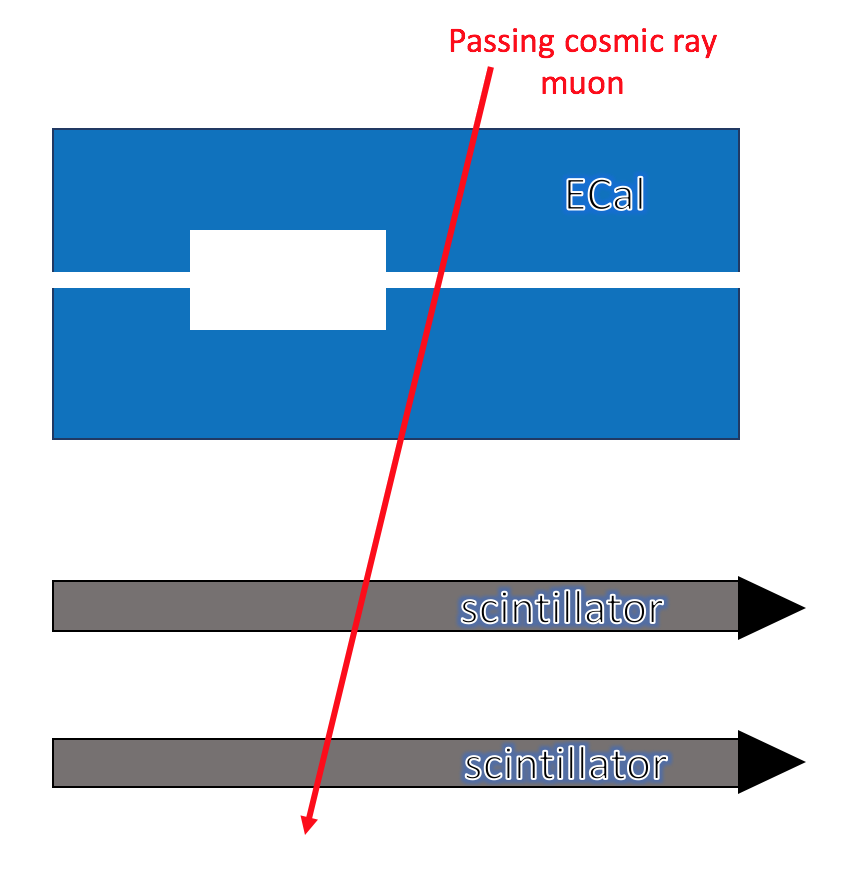
\includegraphics[width=\textwidth]{pics/cosmicSketch.png}
%\end{center}
\end{minipage}\hfill\begin{minipage}{0.45\textwidth}
 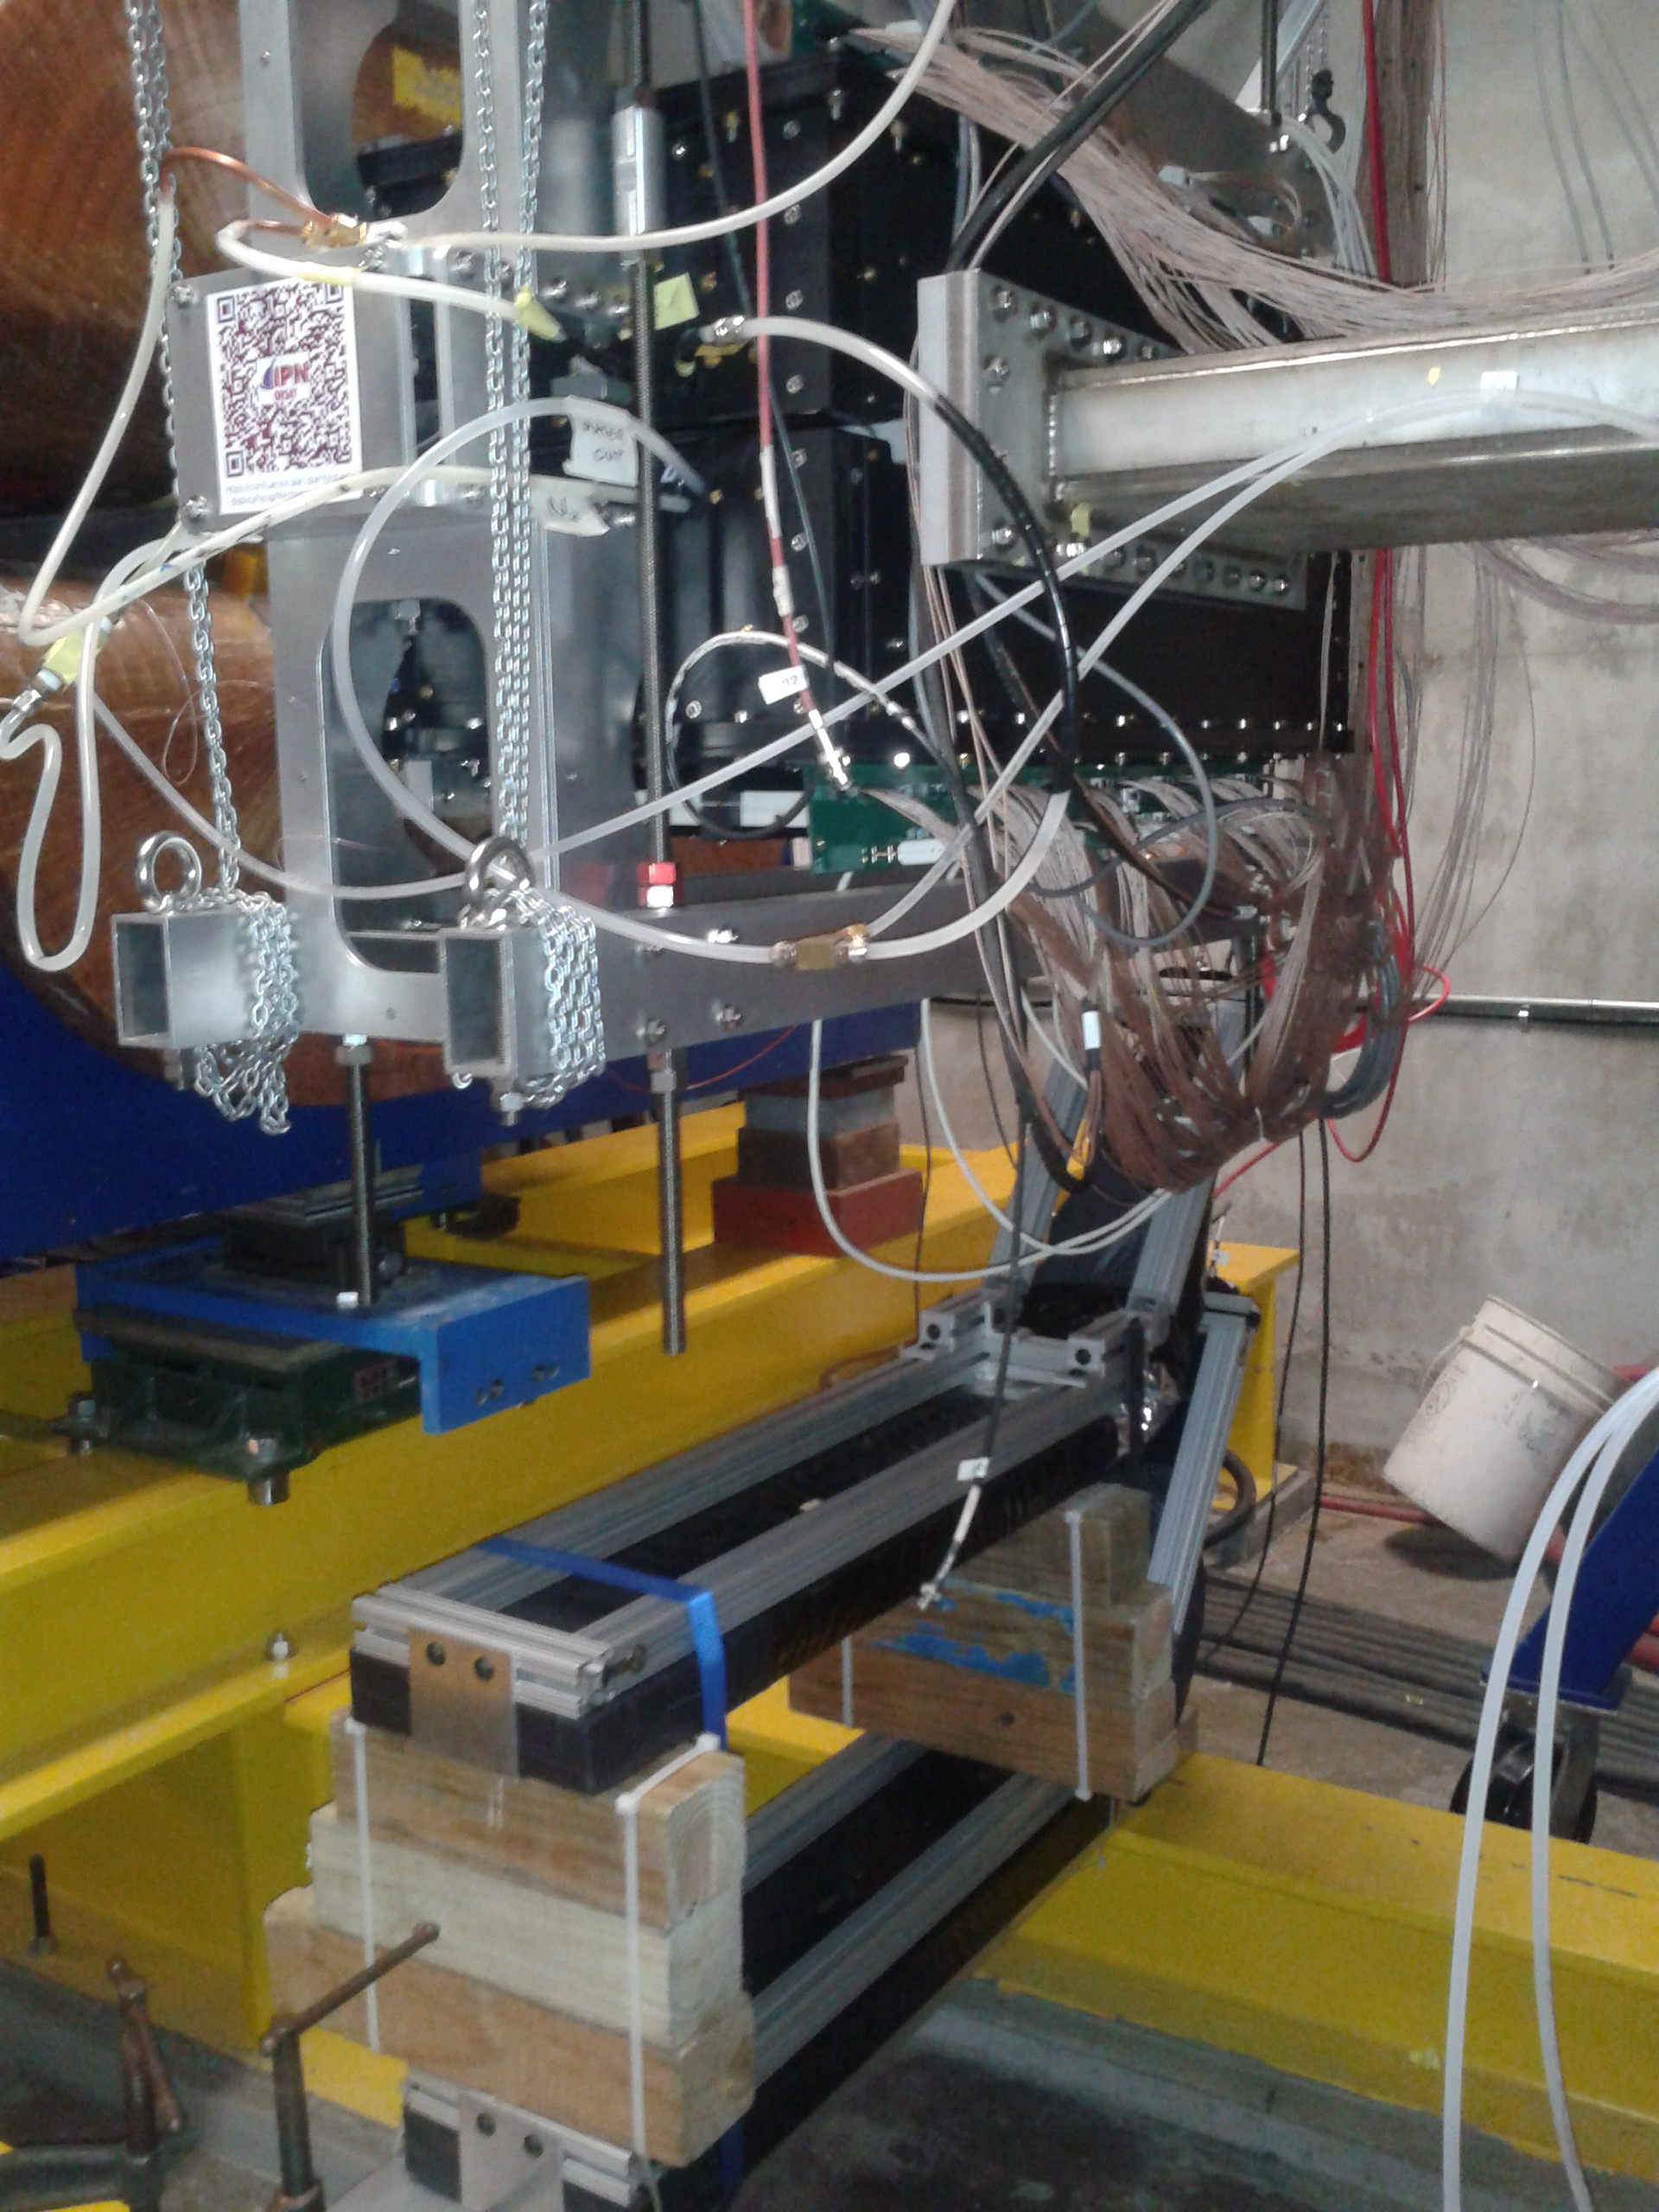
\includegraphics[width=\textwidth]{pics/cosmicPic.jpg}
 \end{minipage}
 \caption[Setup for the cosmic trigger]{A schematic showing the ECal (viewed from downstream) is shown on the left. A cosmic event is triggered when a cosmic ray muon passes vertically through the detector and is detected by both scintillators, located below. The actual installed set up is shown with a similar view from downstream on the right.}
  \label{fig:cosmicSetup}
\end{figure}
Prior to running the ECal with the electron beam, the full detector was able to calibrated using signals from passing cosmic ray muons. These signals were detectable by the ECal due to the upgraded electronics using the large area avalanche photo-diodes. The experimental setup for triggering and reading out cosmic signals in the ECal is shown in Figure~\ref{fig:cosmicSetup}.

The previously used method of calibrating the ECal using cosmic signals is described in \cite{szumila-vance_hps_2016}. An overview is described here. After a cosmic signal is measured from the coincidence of the two triggering scintillators external to the ECal, all 442 modules were read out by the DAQ. The general trigger rate measured at the DAQ was approximately 7~Hz. Offline, a geometric selection of cuts was applied to the data to identify cosmic signals that could be used for calibration. The module of interest was first identified with a threshold crossing in the raw waveform spectra. The cuts required that no threshold crossing in the raw waveform occurred in crystals immediately adjacent in the same row. Further cuts required that adjacent crystals vertically had to have also measured a threshold crossing. If this criteria was met, then the information for that crystal was kept for the calibration.

The calibration procedure selected a window prior to the signal window in the raw FADC wave spectrum to calculate an average event-by-event pedestal for a particular channel. The integral was extracted by summing the raw waveform spectrum in the signal window and subtracting the corresponding pedestal. This pulse-integral was recorded over many events and fit with a Landau-Gaussian convolution. The peak of the fit was obtained numerically and corresponded to the FADC calibration point. The procedure described above will differ from that described by this note. The acquisition of the data will be the same, but the cuts and fits to extract the gain for each module will be different and described in detail. 

%------------------------------------------------
\section{Method}
The calibration procedure that follows was tuned and developed on the cosmic ray data obtained after the removal of the splitters from the readout chain in 2016. The signal amplitudes in the raw FADC waveform were visually larger than those seen when taken with the splitters. Some time was spent in determining an adequate threshold for a clear minimum ionization peak in the data and keeping good events. 

%insert plot of raw spectrum with signal passing vertically through 10 crystals
%\begin{figure}[htb]
%  \centering
%      \includegraphics[width=0.5\textwidth]{changeme.png}
%  \caption{Cosmic ray signal as seen when passing vertically through a column of ten crystals in the ECal.}
%  \label{rawColumn}
%\end{figure}	


%talk about cut selection: threshold, any geometric cuts

%show equation for raw waveform fitting and initialization
%\begin{equation}
%\label{eq:timediff}
%\Delta t = t_{hit}-t_{RF} 
%\end{equation}	

%show some signal fits
%\begin{figure}[htb]
%  \centering
%      \includegraphics[width=0.5\textwidth]{changeme.png}
%  \caption{Fits using Equation~XX are shown when applied to cosmic signals in various crystals.}
%  \label{fitsToCrystals}
%\end{figure}	


%show chi2 distribution
%\begin{figure}[htb]
%  \centering
%      \includegraphics[width=0.5\textwidth]{changeme.png}
%  \caption{The $\chi^2$ distribution of the raw pulse fit to the cosmic ray signal in crystals is shown.}
%  \label{chiSquared}
%\end{figure}	

%------------------------------------------------
\section{Results}
%discuss the number of events required for the cosmic calibration (rates)

%compare the gain numbers with those found before, like a 1D histogram of the percent difference
%\begin{figure}[htb]
%  \centering
%      \includegraphics[width=0.5\textwidth]{changeme.png}
%  \caption{The difference of the gains obtained using the raw spectrum fitting procedure is compared to the gains obtained using the integrated spectrum with geometric cuts.}
%  \label{gainDiff}
%\end{figure}	

%show energy resolution compared to old method
%\begin{figure}[htb]
%  \centering
%      \includegraphics[width=0.5\textwidth]{changeme.png}
%  \caption{The elastically-scattered electron peak is shown with only the calibration from cosmic ray muons.}
%  \label{eseCompare}
%\end{figure}	

%If time, re-calibrate using elastically-scattered electrons and see if there is any improvement to the overally energy resolution


%------------------------------------------------
\section{Conclusion}
%Does this change the cosmic time needed to run?
%Does this improve the resolution of the whole ECal? edge crystals? those not in elastic acceptance?
%Are there other ways to improve the trigger? Maybe using the Ecal...
%include discussion of where to access the software

%----------------------------------------------------------------------------------------
%	REFERENCE LIST
%----------------------------------------------------------------------------------------

\bibliography{biblio}{}
\bibliographystyle{unsrt}


%----------------------------------------------------------------------------------------
\end{document}